\documentclass[11pt]{article}
%\usepackage[firstpage]{draftwatermark}
\usepackage{times}
\usepackage{pdfpages}
\usepackage{fullpage}
\usepackage{url}
\usepackage{hyperref}
\usepackage{fancyhdr}
\usepackage{graphicx}
\usepackage{tabularx}
\usepackage{enumitem}
\usepackage{indentfirst}
\usepackage{subcaption}
\usepackage{amsmath, amsfonts, amsthm, fouriernc}
\usepackage{units}
\usepackage{IEEEtrantools}
\usepackage{parskip}
%\usepackage{multicol}
\usepackage{paracol}

\usepackage{color,soul}
\DeclareRobustCommand{\hlr}[1]{{\sethlcolor{red}\hl{#1}}}
\DeclareRobustCommand{\hlg}[1]{{\sethlcolor{green}\hl{#1}}}
\DeclareRobustCommand{\hlb}[1]{{\sethlcolor{blue}\hl{#1}}}
\DeclareRobustCommand{\hly}[1]{{\sethlcolor{yellow}\hl{#1}}}

\setcounter{secnumdepth}{4}
\graphicspath{{images/}}
\pagestyle{fancy}

\newenvironment{xitemize}{\begin{itemize}\addtolength{\itemsep}{-0.75em}}{\end{itemize}}
\newenvironment{tasklist}{\begin{enumerate}[label=\textbf{\thesubsubsection-\arabic*},ref=\thesubsubsection-\arabic*,leftmargin=*]}{\end{enumerate}}
\newcommand\todo[1]{{\bf TODO: #1}}
\setcounter{tocdepth}{2}
\setcounter{secnumdepth}{4}

\addtolength{\headheight}{2em}
\addtolength{\headsep}{1.5em}
\lhead{\large{ME 2801}}

% This command sets the font size for all \section headings.
% 12 is the font size in points
% 15 is the baseline skip (vertical space between lines) in points
\usepackage{sectsty}
\sectionfont{\fontsize{12}{8}\selectfont}

\begin{document}

\begin{center}
  \Large{\bf{HW 3: Time Response}}
\end{center}

The textbook exercises, designated by with the word “Nise”, are from “Problems” section at the end of the chapter in “Control System Engineering” by Norman Nise, 7th edition.

This assignment uses exercises from the textbook.  The additional instructions are to clarify and/or expand each exercise.

\section*{Nise 4.2 and 4.3: Step response of first-order system}

For the MATLAB plots, add annotation (by hand or using the computer) to indicate the \emph{time-constant} of the system.
 
\section*{Nise 4.8 }

\begin{itemize}
  \item Generate the pole/zero plots 'by hand'; a simple sketch of the s-plane is sufficient
    \begin{itemize}
      \item The MATLAB function \texttt{roots()} is a handy way to find the roots of polynomials (if you want to avoid using the quadratic equation).
      \item Optional: If you would like to check your work, the MATLAB function \texttt{pzmap()} will work directly on the transfer function.
    \end{itemize}
    \item You can use the MATLAB \texttt{step()} command to plot the step response.  This is a good way to check your understanding of poles, zeros, damping, etc.  We are trying to build up some intuition to connect the pole-zero locations with the time response characteristics.
    \item The \emph{general forms} referred to the problem statement are these:
    \begin{IEEEeqnarray*} {rCl}
      c(t) & = & K[1-e^{-at}]  \\
      c(t) & = & K[1-Ae^{-\sigma_1 t}-Be^{-\sigma_2 t}] \\
      c(t) & = & K[1-Ae^{-\sigma_d t} \cos(\omega_d t - \phi)] \\
      c(t) & = & K[1 - A \cos(\omega_1 t - \phi)] \\
      c(t) & = & K[1 - Ae^{-\sigma_1 t} - B \, t \,e^{-\sigma_1 t}] 
    \end{IEEEeqnarray*}
    Without solving for the inverse Laplace transform, you should be able to identify  numeric values for the variables $a, \sigma_1, \sigma_2, \sigma_d, \omega_d, \omega_1, \sigma_1$ from the respective general forms.  You do not need to find the coefficients $K, A, B$.
  \end{itemize}


\section*{Nise 4.20 and 4.21: Response of second-order system}

\subsection*{Nise 4.20}

For calculating the rise time, $T_r$, by hand for an underdamped second order model, 
according to the Nise textbook (7th Ed.) "a precise analytical relationship between rise time and damping ratio cannot be found."  Instead a numerical solution is provided as represented by Nise Figure 4.16".  In a footnote on the same page the textbook as two polynomial fits of the numerical solutions.

For the purposes of the class you may either use Figure 4.16 as a lookup table to approximate $T_r$ for a given model, or use the supplied polynomial expressions.

Figure 4.16 is reproduced here with more resolutions and grid lines to aid in its use as a lookup table.
\begin{figure}[h]
  \centering
  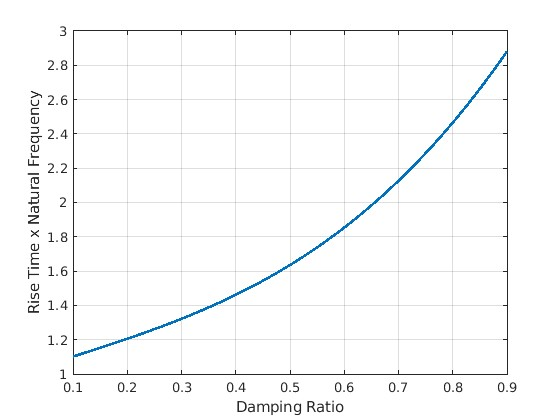
\includegraphics[width=0.7\textwidth]{figure_4_16.jpg}
  \caption{Reproduction of Nise Figure 4.16}
  \label{fig:figure_4_16}
\end{figure}

\subsection*{Nise 4.12}

For the MATLAB portion of the problem the \texttt{stepinfo()} and \texttt{damp()} commands might be useful for investigation the system metrics.

\section*{Nise 4.23: Given performance metrics, find pole locations}

\section*{Nise 4.32}

Check your answers by using MATLAB to plot the step response and verify that the results agree with the graphs in the exercise.


\end{document}


